
\begin{figure} \begin{center}
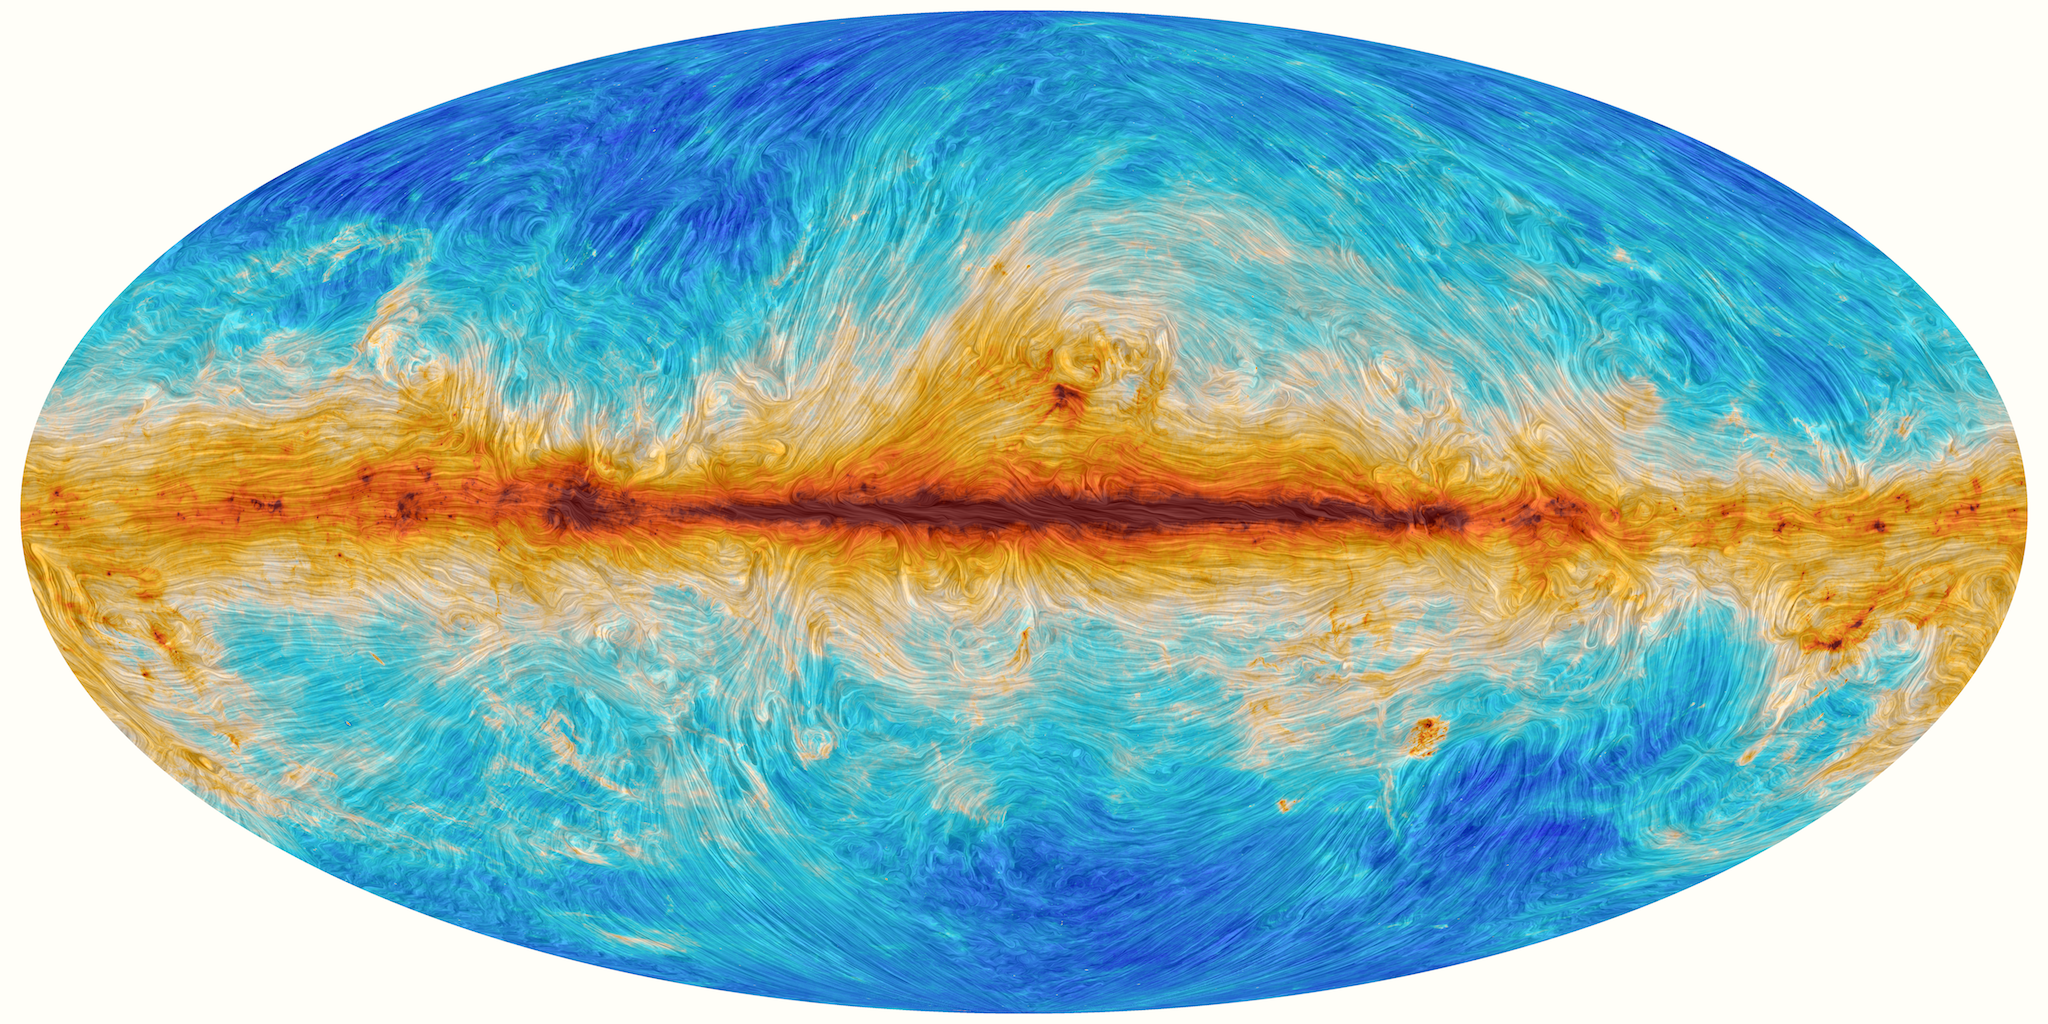
\includegraphics[width=\textwidth]{figs/2015_353GHz_B-field.png}
\caption[ ]{The large scale magnetic field of the galaxy as seen by the Planck
satellite. The color field shows dust emission at 353GHz.  The image is smeared
along the direction of the magnetic field.  \citep{PlanckXIX15}}
\label{fig.PlanckField} \end{center} \end{figure}
